\documentclass[ucs]{beamer}
\usetheme{Frankfurt}
% \usecolortheme{seahorse}

\usepackage[utf8x]{inputenc}
\usepackage[T2A]{fontenc}

\usepackage[english,russian]{babel}
\usepackage{amssymb, amsmath, amsfonts, amsthm}
\usepackage{multirow}
\usepackage{booktabs}
\usepackage{array}
% \usepackage{rotating}
% \usepackage{caption}
\usepackage{pgfmath}
\usepackage{tikz}
\usetikzlibrary{arrows,fit,positioning,shapes.multipart}

\title{Сравнение TVD ограничителей}
\author{Рогозин Олег}
\institute{
	Московский физико-технический институт (государственный университет) \\
	Российский научный центр ``Курчатовский институт''
}

\newcommand{\dd}{\:\mathrm{d}}
\newcommand{\Kn}{\mathrm{Kn}}
\newcommand{\TV}{\mathrm{TV}}

\begin{document}

\frame{\titlepage}
\begin{frame}
	\frametitle{Содержание}
	\tableofcontents
\end{frame}

\section{Уравнение переноса}

\begin{frame}
	\frametitle{Численное решение уравнения переноса}
	\begin{columns}
		\column{.45\textwidth}
		\begin{block}<1->{Уравнение переноса}
			\centering\(f_t+\xi f_x=0, \quad \xi>0 \)
		\end{block}
		\column{.45\textwidth}
		\begin{block}<1->{Точное решение}
			\centering\(f(x,t) = f(x-\xi t,0) \)
		\end{block}
	\end{columns}
	\begin{block}<2->{Шаблоны конечно-разностных схем}
		\centering Проекция на сетку \( f(x,t) = f(ih,n\tau) \rightarrow f_i^n \) \bigskip
		\begin{columns}[totalwidth=\textwidth]
			\column{.25\textwidth}
			\centering левый уголок
			\begin{tikzpicture}[point/.style={shape=circle,draw,fill,minimum size=2mm,inner sep=0, node distance=2cm}, >=latex', thick, scale=1]
				\node[point] (10) at (0,0) {};
				\node[below] at (10.south) {\(f_i^n\)};
				\node[point] (00) at (-1,0) {};
				\node[below] at (00.south) {\(f_{i-1}^n\)};
				\node[point] (11) at (0,1) {};
				\node[above] at (11.north) {\(f_i^{n+1}\)};
				\draw[-] (10) to (00);
				\draw[-] (10) to (11);
			\end{tikzpicture}
			\column{.3\textwidth}
			\centering Лакс"--~Вендрофф
			\begin{tikzpicture}[point/.style={shape=circle,draw,fill,minimum size=2mm,inner sep=0, node distance=2cm}, >=latex', thick, scale=1]
				\node[point] (20) at (1,0) {};
				\node[below] at (20.south) {\(f_{i+1}^n\)};
				\node[point] (10) at (0,0) {};
				\node[below] at (10.south) {\(f_i^n\)};
				\node[point] (00) at (-1,0) {};
				\node[below] at (00.south) {\(f_{i-1}^n\)};
				\node[point] (11) at (0,1) {};
				\node[above] at (11.north) {\(f_i^{n+1}\)};
				\draw[-] (10) to (00);
				\draw[-] (10) to (20);
				\draw[-] (10) to (11);
			\end{tikzpicture}
			\column{.35\textwidth}
			\centering TVD схемы
			\begin{tikzpicture}[point/.style={shape=circle,draw,fill,minimum size=2mm,inner sep=0, node distance=2cm}, >=latex', thick, scale=1]
				\node[point] (30) at (-2,0) {};
				\node[below] at (30.south) {\(f_{i-2}^n\)};
				\node[point] (20) at (1,0) {};
				\node[below] at (20.south) {\(f_{i+1}^n\)};
				\node[point] (10) at (0,0) {};
				\node[below] at (10.south) {\(f_i^n\)};
				\node[point] (00) at (-1,0) {};
				\node[below] at (00.south) {\(f_{i-1}^n\)};
				\node[point] (11) at (0,1) {};
				\node[above] at (11.north) {\(f_i^{n+1}\)};
				\draw[-] (10) to (00);
				\draw[-] (10) to (20);
				\draw[-] (10) to (30);
				\draw[-] (10) to (11);
			\end{tikzpicture}
		\end{columns}
	\end{block}
\end{frame}

\begin{frame}
	\frametitle{Требования к разностным схемам}
	\setbeamertemplate{items}[circle]
	\setbeamerfont{item projected}{size=\huge}
	\setbeamerfont{itemize/enumerate body}{size=\huge}
	\begin{enumerate}
		\item Сходимость \bigskip
		\item Консервативность \bigskip
		\item Монотонность \bigskip
		\item Второй порядок
	\end{enumerate}

\end{frame}

\begin{frame}
	\frametitle{Метод коррекции потоков}
	\begin{block}{Flux-Corrected Transport // Jay Boris \& David Book --- 1973}
		\[ f_i^{n+1} = f_i^n - \gamma\left(f_{i+\frac1{2}}^n-f_{i-\frac1{2}}^n\right) \]
		\[ f_{i+\frac1{2}} = f_i + \frac{1-\gamma}{2}\varphi(\theta_i)(f_{i+1} - f_i) \]
		\centering
		\begin{tikzpicture}[point/.style={shape=circle,draw,fill,minimum size=2mm,inner sep=0,node distance=2cm},
							red/.style={thin,color=red,->}, blue/.style={thin,color=blue,->},
							>=latex', thick, scale=1.5]
			\node[point] (30) at (-2,0) {};
			\node[point] (20) at (1,0) {};
			\node[point] (10) at (0,0) {};
			\node[point] (00) at (-1,0) {};
			\node[point] (11) at (0,1) {};
			\node[red] (l) at (-.5,.5) {\(\times\)};
			\node[blue] (r) at (.5,.5) {\(\times\)};
			\node[above left] at (l) {\(f_{i-\frac1{2}}\)};
			\node[above right] at (r) {\(f_{i+\frac1{2}}\)};
			\draw[-] (10) to (00); \draw[-] (10) to (20); \draw[-] (10) to (30); \draw[-] (10) to (11);
			\draw[red] (11) to (l); \draw[red] (l) to (10); \draw[red] (l) to (00); \draw[red] (l) to (30);
			\draw[blue] (11) to (r); \draw[blue] (r) to (10); \draw[blue] (r) to (00); \draw[blue] (r) to (20);
		\end{tikzpicture} \\
	\vspace{.5cm}
	\end{block}
	Число Куранта CFL (\emph{Courant"--~Friedrichs"--~Lewy}) \( \gamma=\dfrac{\xi\tau}{h} \) \\
	Ограничитель (\emph{limiter}) \(\varphi(\theta)\) \\
	Показатель гладкости решения \(\theta_i = \dfrac{f_i - f_{i-1}}{f_{i+1} - f_i} = 1-h\dfrac{f_{xx}}{f_x}+\mathcal{O}(h^2)\)
\end{frame}

\begin{frame}
	\frametitle{Метод Рунге"--~Кутты}
	\begin{block}<1->{Решение задачи Коши}
		\[ f_t = L(f) \]
		\[ L(f_i) = - \frac{\xi}{h}\left(f_{i+\frac1{2}}-f_{i-\frac1{2}}\right) \]
		\[ f_{i+\frac1{2}} = f_i + \frac1{2}\varphi(\theta_i)(f_{i+1} - f_i) \]
	\end{block}
	\begin{block}<2->{}
		\centering Обе схемы устойчивы при \(\gamma < 1\)
	\end{block}
\end{frame}

\begin{frame}
	\frametitle{REA (reconstruct-evolve-average)}
	\begin{columns}
		\column{.6\textwidth}
		\begin{block}<1->{Кусочно-линейная аппроксимация}
			\[ f(x,t_n) = f_i^n + \sigma_i^n(x-x_i) \]
			\[ f_{i+\frac1{2}} = f_i + \frac{1-\gamma}{2}\sigma_ih \]
			\[ \sigma_ih = \varphi(\theta_i)(f_{i+1} - f_i) \]
		\end{block}
		\begin{block}<3->{Следовательно}
			\begin{itemize}
				\item положительный наклон \(\varphi(\theta)>0\) \\
				\item в экстремумах \(\varphi(\theta<0)=0\) \\
			\end{itemize}
		\end{block}
		\pause[2]
		\column{.4\textwidth}
			\begin{tikzpicture}[point/.style={shape=circle,draw,fill,minimum size=2mm,inner sep=0, node distance=2cm},
								back/.style={draw=gray!20,fill=gray!20}, >=latex', very thick, scale=1]
				\draw[back] (.5,-1) -- (.5,-.2) -- (1.5,.2) -- (1.5,-1) -- cycle;
				\draw[back] (1.5,-1) -- (1.5,0) -- (2.5,2) -- (2.5,-1) -- cycle;
				\draw[back] (2.5,-1) -- (2.5,2.4) -- (3.5,2.6) -- (3.5,-1) -- cycle;
				\draw[back] (3.5,-1) -- (3.5,2.4) -- (4.5,1.6) -- (4.5,-1) -- cycle;
				\node[point] (p1) at (1,0) {}; \node[point] (p2) at (2,1) {}; \node[point] (p3) at (3,2.5) {}; \node[point] (p4) at (4,2) {};
				\draw[-] (.5,-.2) to (1.5,.2); \draw[-] (1.5,0) to (2.5,2); \draw[-] (2.5,2.4) to (3.5,2.6); \draw[-] (3.5,2.4) to (4.5,1.6);
				\foreach \x in {0.5,1.5,2.5,3.5,4.5} \draw[dashed] (\x,-1) to (\x,3);
			\end{tikzpicture}
	\end{columns}
\end{frame}

\begin{frame}
	\frametitle{TVD схемы второго порядка}
	\begin{columns}
		\column{.3\textwidth}
		\begin{block}<1->{Второй порядок}
			\[ \lim_{\theta\to1}{\varphi(\theta)} = 1 \] \[ \exists \lim_{\theta\to1}{\varphi'(\theta)} \]
		\end{block}
		\column{.7\textwidth}
		\begin{block}<2->{TVD схема}
			\[ \TV^{n+1}\le \TV^n, \quad \TV^n = \sum_i| f_{i+1}^n - f_i^n | \]
			\centering\emph{явная TVD схема монотонна}\\\smallskip
		\end{block}
	\end{columns}
		\begin{block}<3->{Монотонность}
			\[ |\varphi(\theta)| \leq \mathrm{minmod}\left(\frac2{\gamma}\theta,\frac2{1-\gamma}\right) \]
			\[
			\mathrm{minmod}\,(a,b) \equiv \left\{
			\begin{array}{l l}
				a & \quad \text{if}\;|a|<|b| \;\text{and}\;ab>0, \\
				b & \quad \text{if}\;|b|<|a| \;\text{and}\;ab>0, \\
				0 & \quad \text{if}\;ab \leq 0.
			\end{array}\right.
			\]
			\[ \forall \gamma \; |\varphi(\theta)| \leq \mathrm{minmod}\left(2\theta,2\right) \]
		\end{block}
\end{frame}

\section{Описание ограничителей}

\begin{frame}
	\frametitle{Список ограничителей}
	\framesubtitle{Классические схемы}
	\renewcommand\arraystretch{1.5}
	\begin{table}
		\begin{tabular}{>{\centering}p{3cm}|>{\centering}p{3cm}}
			\toprule
			Название		&  Лимитер \( \varphi(\theta) \) \tabularnewline
			\midrule
			первый порядок	& \( 0 \) \tabularnewline
			Lax"--~Wendroff	& \( 1 \) \tabularnewline
			Fromm			& \( \dfrac{1+\theta}2 \) \tabularnewline
			Beam"--~Warming	& \( \theta \) \tabularnewline
			\bottomrule
		\end{tabular}
	\end{table}
\end{frame}

\begin{frame}
	\frametitle{Список ограничителей}
	\framesubtitle{TVD схемы}
	\begin{table}
		\begin{tabular}{>{\centering}p{3cm}|>{\centering}p{6cm}}
			\toprule
			Название			&  Лимитер \( \varphi(\theta) \) \tabularnewline
			\midrule
			minmod			& \( \min\left(\theta,1\right) \) \tabularnewline
			MC 				& \( \min\left(2\theta,\dfrac{1+\theta}{2},2\right) \) \tabularnewline
			Koren 			& \( \min\left(2\theta,\dfrac{2+\theta}{3},2\right) \) \tabularnewline
			superbee		 	& \( \max(\min(2\theta,1),\min(\theta,2)) \) \tabularnewline
			van Leer			& \( \dfrac{2\theta}{1+\theta} \) \tabularnewline
			van Albada		& \( \dfrac{2\theta}{1+\theta^2} \) \tabularnewline
			\midrule
			wide superbee 	& \( \max\left(\min\left(\dfrac2{\gamma}\theta,1\right),\min\left(\theta,\dfrac2{1-\gamma}\right)\right) \) \tabularnewline
			wide third order	& \( \min\left(\dfrac2{\gamma}\theta,\dfrac{(\gamma+1)\theta+(2-\gamma)}{3},\dfrac2{1-\gamma}\right) \) \tabularnewline
			\bottomrule
		\end{tabular}
	\end{table}
\end{frame}

\begin{frame}
	\frametitle{Список ограничителей}
	\framesubtitle{Схема Рунге-Кутты третьего порядка}
	\begin{columns}
		\column{.6\textwidth}
		\begin{block}<1->{3 порядок по пространству}
			\centering
			Ограничитель \textit{Koren}
			\[ \varphi(\theta>0) = \mathrm{minmod} \left(2\theta,\dfrac{2+\theta}{3},2\right) \]
		\end{block}
		\column{.4\textwidth}
		\begin{block}<2->{3 порядок по времени}
			\centering
			Схема Хойна \\ (таблица Бутчера) \\ \smallskip
			\begin{tabular}{| c | c | c | c |}
				\hline
				0 & & & \\ \hline
				\(\frac{1}{3}\) & \(\frac{1}{3}\) & & \\ \hline
				\(\frac{2}{3}\) & 0 & \(\frac{2}{3}\) & \\ \hline
				& \(\frac{1}{4}\) & 0 & \(\frac{3}{4}\) \\ \hline
			\end{tabular}
		\end{block}
	\end{columns}
	
\end{frame}

\begin{frame}
	\frametitle{Диаграмма Sweby}
	\framesubtitle{Классические схемы и их линейные комбинации, ограниченные условием TVD}
	\begin{center}
		\begin{tikzpicture}[>=latex',thick, scale=1.5, domain=0:4]
			\draw[draw=gray!20,fill=gray!20] (0,0) -- (1,2) -- (4.1,2) -- (4.1,0) -- cycle;
			\node[above] at (.8,0) {TVD};
			\draw[<->] (4.2,0) node[right] {\(\theta\)} -- (0,0) -- (0,2.7) node[above] {\(\varphi(\theta)\)};
			\foreach \x in {0,1,2,3,4}
				\draw (\x cm,1pt) -- (\x cm,-1pt) node[anchor=north] {\(\x\)};
			\foreach \y in {0,1,2}
				\draw (1pt,\y cm) -- (-1pt,\y cm) node[anchor=east] {\(\y\)};
			\node[draw,circle,minimum size=.3cm] (sec) at (1,1) {};
			\node[text width=1cm,text centered] (cap) at (0.8,1.7) {second order};
			\draw[->] (cap.south) to (sec);

			\draw[color=purple!50!blue] (0,0) -- (0.25,0.5) -- (2.5,2) -- (2.7,2) node[above] {Koren} -- (4,2);
			\draw[color=green!50!black] (0,0) -- (0.333,0.667) -- (3,2) node[below right] {MC} -- (4,2);
			\draw[color=blue] (-.1,-.1) -- (2.2,2.2) node[above left] {Beam"--~Warming} -- (2.9,2.9);
			\draw[dashed,color=green] (-.1,.45) -- (4,2.5) node[above left] {Fromm};
			\draw[color=red] (-.1,1) -- (2.5,1) node[below right] {Lax"--~Wendroff} -- (4,1);
		\end{tikzpicture}
	\end{center}
\end{frame}

\begin{frame}
	\frametitle{Диаграмма Sweby}
	\framesubtitle{Другие нелинейные лимитеры}
	\begin{center}
		\begin{tikzpicture}[>=latex',thick, scale=1.5, domain=0:4]
			\draw[draw=gray!20,fill=gray!20] (0,0) -- (1,2) -- (4.1,2) -- (4.1,0) -- cycle;
			\node[above] at (.8,0) {TVD};
			\draw[<->] (4.2,0) node[right] {\(\theta\)} -- (0,0) -- (0,2.7) node[above] {\(\varphi(\theta)\)};
			\foreach \x in {0,1,2,3,4}
				\draw (\x cm,1pt) -- (\x cm,-1pt) node[anchor=north] {\(\x\)};
			\foreach \y in {0,1,2}
				\draw (1pt,\y cm) -- (-1pt,\y cm) node[anchor=east] {\(\y\)};
			\node[draw,circle,minimum size=.3cm] (sec) at (1,1) {};
			\node[text width=1cm,text centered] (cap) at (0.8,1.7) {second order};
			\draw[->] (cap.south) to (sec);

			\draw[color=blue] (0,0) -- (1,1) -- (4,1) node[below left] {minmod};
			\draw[color=green!50!black] (0,0) -- (.5,1) -- (1,1) -- (2,2) -- (4,2) node[above left] {superbee};
			\draw[color=purple!50!blue,smooth] plot[id=leer] function{(2*x)/(1+x)} node[below left] {van Leer};
			\draw[color=olive,smooth] plot[id=albada] function{(2*x)/(1+x*x)} node[below left] {van Albada};
		\end{tikzpicture}
	\end{center}
\end{frame}

\begin{frame}
	\frametitle{Диаграмма Sweby}
	\framesubtitle{Улучшенные лимитеры, зависящие от числа Куранта \(\gamma\)}
	\begin{center}
		\begin{tikzpicture}[>=latex',thick, scale=1, domain=0:4]
			\draw[draw=gray!10,fill=gray!10] (0,0) -- (.5,3) -- (6.1,3) -- (6.1,0) -- cycle;
			\draw[draw=gray!20,fill=gray!20] (0,0) -- (1,2) -- (6.1,2) -- (6.1,0) -- cycle;
			\node[below] at (1.5,3) {TVD \(\gamma=\frac1{3}\)};
			\node[above] at (1,0) {TVD \(\forall\gamma\)};
			\draw[<->] (6.3,0) node[right] {\(\theta\)} -- (0,0) -- (0,3.5) node[above] {\(\varphi(\theta)\)};
			\foreach \x in {0,1,2,3,4,5,6}
				\draw (\x cm,1pt) -- (\x cm,-1pt) node[anchor=north] {\(\x\)};
			\foreach \y in {0,1,2,3}
				\draw (1pt,\y cm) -- (-1pt,\y cm) node[anchor=east] {\(\y\)};
			\node[draw,circle,minimum size=.3cm] (sec) at (1,1) {};
			\node[text width=1cm,text centered] (cap) at (3,.8) {second order};
			\draw[->] (cap.west) to (sec);

			\draw[color=red] (0,0) -- (.1666,1) -- (1,1) -- (3,3) -- (4,3) node[above] {superbee (\(\gamma={}^1/_3\))} -- (6,3);
			\draw[color=blue] (0,0) -- (.1,.6) -- (3,1.888) node[below right] {third (\(\gamma={}^1/_3\))} -- (5.5,3) -- (6,3);
		\end{tikzpicture}
	\end{center}
\end{frame}

\section{Сравнение лимитеров}

\begin{frame}
	\frametitle{Визуальное сравнение}
	\begin{columns}
		\column{.5\textwidth}
		\centering{first}\\
		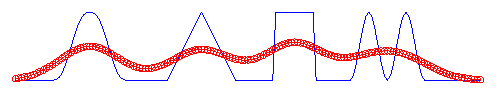
\includegraphics[width=\textwidth]{conver/first}\\
		\pause[2]
		\centering{Lax"--~Wendroff}\\
		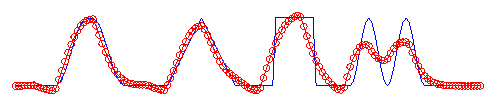
\includegraphics[width=\textwidth]{conver/lw}\\
		\centering{Beam"--~Warming}\\
		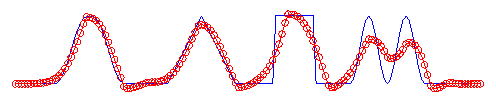
\includegraphics[width=\textwidth]{conver/bw}\\
		\centering{Fromm}\\
		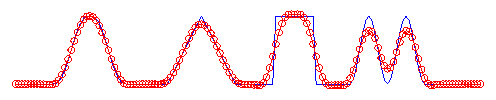
\includegraphics[width=\textwidth]{conver/fromm}\\
		\column{.5\textwidth}
		\pause[3]
		\centering{minmod}\\
		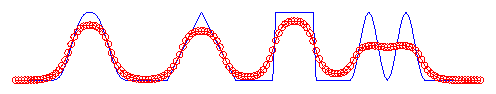
\includegraphics[width=\textwidth]{conver/minmod}\\
		\pause[4]
		\centering{van Albada}\\
		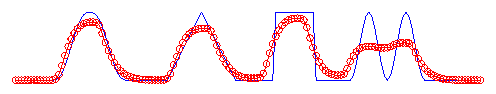
\includegraphics[width=\textwidth]{conver/vanalbada}\\
		\centering{van Leer}\\
		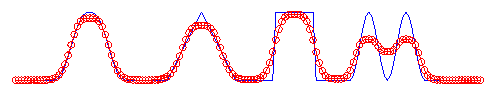
\includegraphics[width=\textwidth]{conver/vanleer}\\
		\centering{Koren}\\
		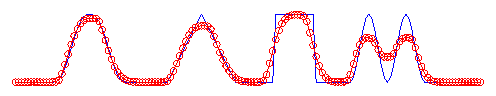
\includegraphics[width=\textwidth]{conver/koren}\\
	\end{columns}
\end{frame}

\begin{frame}
	\frametitle{Визуальное сравнение}
	\begin{columns}
		\column{.5\textwidth}
		\centering{MC}\\
		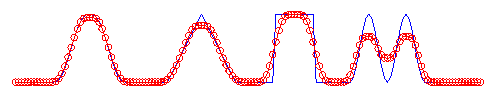
\includegraphics[width=\textwidth]{conver/mc}\\
		\centering{superbee}\\
		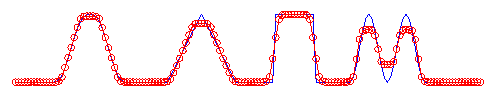
\includegraphics[width=\textwidth]{conver/superbee}\\
		\pause[2]
		\centering{Runge"--~Kutta + Koren}\\
		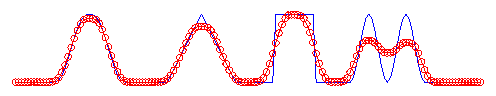
\includegraphics[width=\textwidth]{conver/runge}\\
		\column{.5\textwidth}
		\pause[3]
		\centering{wide superbee}\\
		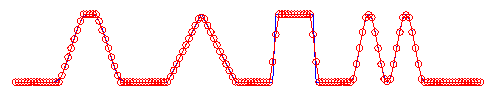
\includegraphics[width=\textwidth]{conver/superbee_g}\\
		\centering{wide third}\\
		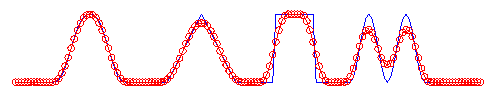
\includegraphics[width=\textwidth]{conver/third_g}\\
	\end{columns}
\end{frame}

\begin{frame}
	\frametitle{Численное сравнение}
	\framesubtitle{Порядок сходимости}
	Для численного сравнения лимитеров использовалась октаэдрическая норма:
	\[ D(M) = \|f-v\| = \frac1{M}\sum_{i=1}^{M}|f_i-v_i| = \mathcal{O}(h^q) \]
	Порядок сходимости:
	\[ q = \log_2\frac{D(M)}{D(2M)} \]
	Моделировались следующие функции:
	\begin{alignat*}{2}
		g_0(x) &= 1,\quad &|x| < 1, \\
		g_1(x) &= 1-|x|,\quad &|x| < 1, \\
		g_2(x) &= 1-3|x|^2+2|x|^3,\quad &|x| < 1, \\
		g_3(x) &= 1-10|x|^3+15|x|^4-6|x|^5,&\quad |x| < 1. 
	\end{alignat*}

\end{frame}

\begin{frame}
	\frametitle{Численное сравнение}
	\framesubtitle{Порядок сходимости}
	\scriptsize
	\begin{tabular}{|l|c|c|c|c||c|c|c|c|}
		\hline
		\multirow{2}{*}{Лимитер} & \multicolumn{4}{c||}{\(\gamma=0.5\)} & \multicolumn{4}{c|}{\(\gamma=0.9\)} \\ \cline{2-9}
		& \(\nexists f\) & \(\nexists f'\) & \(\nexists f''\) & \(\nexists f'''\) 
		& \(\nexists f\) & \(\nexists f'\) & \(\nexists f''\) & \(\nexists f'''\) \\ \hline
		first order				& 0.500 & 1.000 & 0.991 & 0.983 & 0.500 & 1.000 & 0.998 & 0.997 \\ \hline
		Lax"--~Wendroff			& 0.674 & 1.280 & 1.956 & 1.993 & 0.582 & 1.233 & 1.964 & 1.999 \\ \hline
		Beam"--~Warming			& 0.674 & 1.280 & 1.956 & 1.993 & 0.668 & 1.291 & 1.986 & 1.999 \\ \hline
		Fromm					& 0.765 & 1.505 & \color{magenta}2.520 & \color{magenta}2.950 & 0.619 & 1.282 & 1.978 & 1.998 \\ \hline
		minmod					& 0.662 & 1.325 & 1.925 & 1.982 & 0.658 & 1.322 & 1.940 & 1.990 \\ \hline
		van Albada				& 0.675 & 1.323 & 1.954 & 1.999 & 0.670 & 1.307 & 1.967 & 1.999 \\ \hline
		van Leer				& 0.747 & 1.486 & \color{magenta}2.212 & \color{magenta}2.933 & 0.707 & 1.414 & 2.033 & 2.002 \\ \hline
		Koren					& 0.667 & 1.333 & 1.964 & 2.000 & 0.660 & 1.305 & 1.967 & 2.000 \\ \hline
		MC						& 0.752 & 1.534 & \color{magenta}2.424 & \color{magenta}2.931 & 0.691 & 1.397 & 1.991 & 2.000 \\ \hline
		superbee				& \color{olive}1.000 & 1.519 & 1.933 & 2.000 & \color{olive}0.997 & 1.500 & 1.961 & 2.000 \\ \hline
		wide superbee			& \color{olive}1.000 & 1.694 & 1.933 & 2.000 & \color{olive}1.000 & \(\sim\)1.7 & 1.959 & 2.000 \\ \hline
	\color{magenta}	wide third	& 0.749 & 1.508 & \color{magenta}2.597 & \color{magenta}2.918 & 0.747 & 1.534 & \color{magenta}2.530 & \color{magenta}2.947 \\ \hline
	\color{magenta}	RK3+Koren	& 0.753 & 1.541 & \color{magenta}2.445 & \color{magenta}2.905 & 0.751 & 1.511 & \color{magenta}2.428 & \color{magenta}2.899 \\ \hline
	\end{tabular}
\end{frame}

\begin{frame}
	\frametitle{Численное сравнение}
	\framesubtitle{Значение невязки}
	\begin{center}
		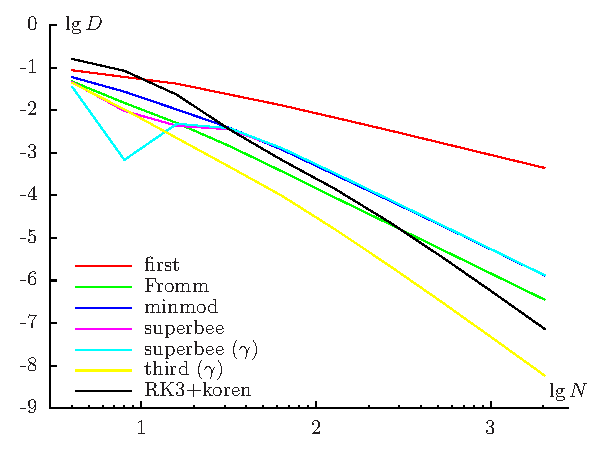
\includegraphics[width=.8\textwidth]{residual/09_3dis}\\
		\(\gamma=0.9\) для гладкой функции
	\end{center}
\end{frame}

\begin{frame}
	\frametitle{Задача теплопроводности}
	\centering{Зависимость потока массы от координаты} \\
	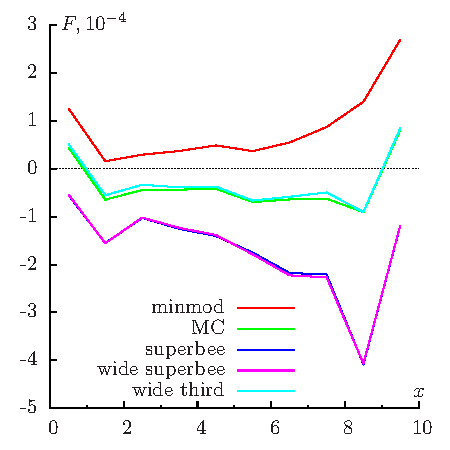
\includegraphics[width=.5\textwidth]{rare_flow}
	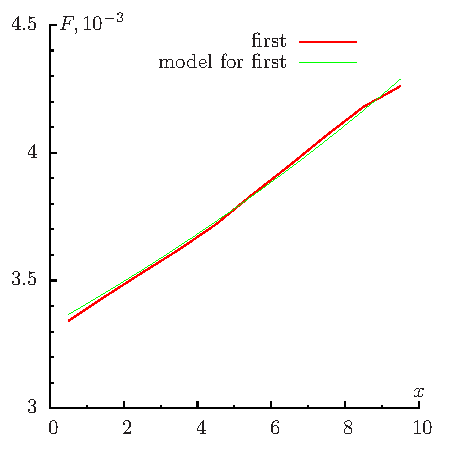
\includegraphics[width=.5\textwidth]{rare_first}
\end{frame}

\begin{frame}
	\frametitle{Структура ударной волны}
	\centering
	 \begin{center}
	    Профили температуры и плотности (\(M=3\)) \\
	    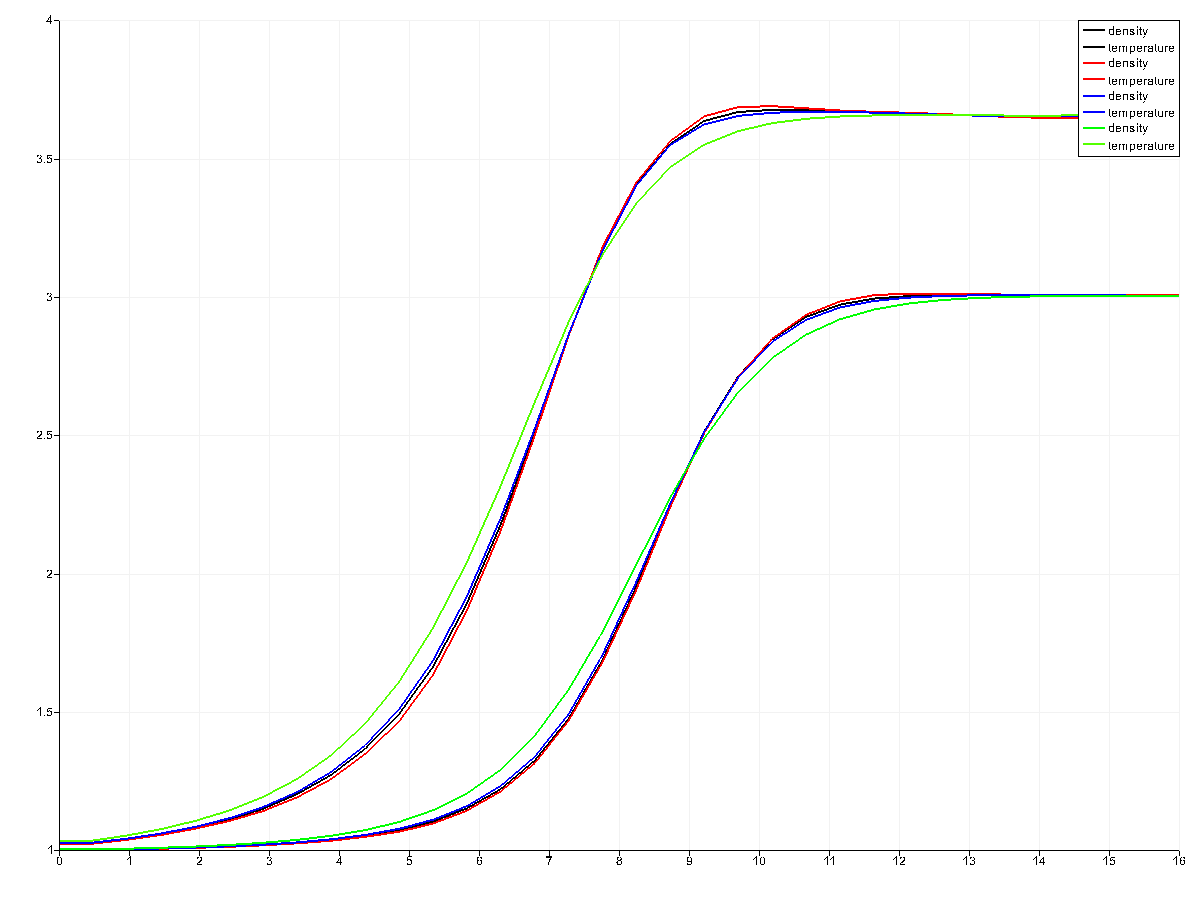
\includegraphics[width=.8\textwidth]{shock}
	 \end{center}
 
\end{frame}

\section*{}
\begin{frame}
	\frametitle{Заключение}
	Для решения кинетического уравнения Больцмана предлагается использовать два различных ограничителя:
	\begin{itemize}
		\item для \alert{грубых} сеток и \alert{разрывных} решений \alert{wide superbee}
			\[ \varphi(\theta,\gamma) = \max\left(\min\left(\dfrac2{\gamma}\theta,1\right),\min\left(\theta,\dfrac2{1-\gamma}\right)\right) \] \\
		\item для \alert{гладких} решений \alert{wide third} 
			\[ \varphi(\theta,\gamma) = \min\left(\dfrac2{\gamma}\theta,\dfrac{(\gamma+1)\theta+(2-\gamma)}{3},\dfrac2{1-\gamma}\right) \] \\
	\end{itemize}

\end{frame}

\end{document}
